% !TEX program = pdflatex
\documentclass[12pt,a4paper]{article}

% --- Packages for the English language (no Cyrillic needed) ---
\usepackage[utf8]{inputenc}
\usepackage[T1]{fontenc}
\usepackage[english]{babel}
% -------------------------------------------------
\usepackage{amsmath,amssymb,amsfonts,mathtools}
\DeclareMathOperator{\Tr}{Tr}

\usepackage{amsmath,amssymb,amsfonts,mathtools}
\usepackage{geometry}
\geometry{left=2cm,right=2cm,top=2cm,bottom=2cm}
\usepackage{booktabs}
\usepackage{array}
\usepackage{hyperref}
\usepackage{url}
\usepackage{xcolor}
\usepackage{titlesec}
\usepackage{fancyhdr}
\usepackage{enumitem}
\usepackage{tikz}
\usetikzlibrary{arrows.meta, positioning, calc, shapes.geometric, decorations.pathreplacing}

% Theorems
\newtheorem{theorem}{Theorem}
\newtheorem{remark}{Remark}

\hypersetup{
	colorlinks=true,
	linkcolor=blue,
	citecolor=blue,
	urlcolor=blue,
}

\titleformat{\section}{\Large\bfseries}{\thesection}{1em}{}
\titleformat{\subsection}{\large\bfseries}{\thesubsection}{1em}{}

\begin{document}
	
	\begin{titlepage}
		\centering
		\vspace*{1cm}
		
		{\Huge\bfseries Decentralized YPSDC (d‑YPSDC)\par}
		\vspace{0.3cm}
		{\Large\bfseries Coordination without Direct Communication\\ via a Shared Environmental Index\par}
		\vspace{1cm}
		
		{\large Alexey V. Yakushev\par}
		\vspace{0.3cm}
		{\normalsize Yakushev Research, \url{https://yuct.org/}\par}
		
		\vspace{1.0cm}
		
		{\normalsize Version 1.0, May 2026\par}
		
		\vfill
		
		\begin{abstract}
			\noindent
			The classical YPSDC protocol assumes a centralized topology: one agent actively transmits a short index to another, and both use an \emph{a priori} dictionary to trigger a complex coordinated action. However, systems in which coordination is achieved without any direct exchange of indices are widespread in nature and technology. In this note we formalize the \textbf{decentralized YPSDC (d‑YPSDC)} — a protocol in which all agents simultaneously read the same index from a shared environment, using a pre‑distributed dictionary. Communication between the agents is entirely absent, yet a coordination efficiency \(K_{\mathrm{eff}} \gg 1\) is attained through the simultaneity of access to the environmental index. We discuss manifestations of d‑YPSDC in biology (flocking behavior), economics (market reaction to macroeconomic indicators), computer science (blockchain oracles), and fundamental physics (quantum non‑locality). The model points to the existence of a deep \textbf{coordination field} that serves as a universal carrier of indices and activates the shared dictionary of the laws of nature.
		\end{abstract}
		
		\vspace{1cm}
		\textcopyright\ 2026 Alexey V. Yakushev. All rights reserved.
	\end{titlepage}
	
	\tableofcontents
	\newpage
	
	\section{Introduction: From Centralized YPSDC to a Decentralized Protocol}
	
	The classical YPSDC (Yakushev Protocol for Synchronous Distributed Coordination) describes the coordination of two or more agents, one of which \textbf{actively transmits} a short index, while the others \textbf{receive} it and activate a complex entry from a shared \emph{a priori} dictionary \cite{YUCT}. In such a scheme there is always a distinguished sender, and the interaction topology is “point‑to‑point” or “star.”
	
	Observations of biological, social, and physical systems reveal a broad class of phenomena in which coordination is not accompanied by a direct exchange of indices. Birds in a flock change direction simultaneously without a visible leader; the market reacts instantly to the release of a macroeconomic figure; entangled quantum particles exhibit correlations without exchanging signals. In all these cases coordination is achieved because \textbf{all agents simultaneously read the same index from the surrounding environment}, relying on a previously agreed‑upon dictionary.
	
	The purpose of this note is to formalize this mechanism as the \textbf{decentralized YPSDC (d‑YPSDC)}, discuss its mathematical structure, and show that it is a natural generalization of the classical protocol to systems with a “common bus” topology.
	
	\section{Formal Model of d‑YPSDC}
	
	\subsection{Components}
	
	Let the system consist of the following components:
	
	\begin{itemize}[leftmargin=*]
		\item \(\mathcal{A} = \{A_1, A_2, \dots, A_N\}\) — the set of agents (observers, cells, animals, network nodes).
		\item \(\mathcal{D}\) — the \textbf{a‑priori dictionary}, common to all agents and distributed during the offline phase. The dictionary is a set of pairs \(\{ \kappa \to \text{Action} \}\), where \(\kappa\) is a possible index and \(\text{Action}\) is the coordinated action.
		\item \(\mathcal{E}\) — the space of environmental states.
		\item \(S(t) \in \mathcal{E}\) — the \textbf{environmental index}, simultaneously accessible to all agents. The environment is \emph{not} an active sender; it merely provides a physical carrier for the index.
	\end{itemize}
	
	\subsection{Protocol}
	
	\begin{enumerate}[leftmargin=*, label=\textbf{Phase \arabic*:}]
		\item \textbf{Offline dictionary distribution.} The complete dictionary \(\mathcal{D}\) is communicated to all agents in some way (genetically, culturally, or during an initialization step).
		\item \textbf{Online index reading.} At time \(t\) the environment generates the index \(\kappa = S(t)\), which reaches all agents without delay.
		\item \textbf{Activation.} Each agent \(A_i\) independently retrieves the entry \(\mathcal{D}(\kappa)\) from the dictionary and performs the prescribed action. No messages are exchanged among the agents.
	\end{enumerate}
	
	\subsection{Coordination efficiency}
	
	In analogy with the classical YPSDC, the coordination efficiency is defined as the ratio of the entropy of the triggered action to the entropy of the index:
	\begin{equation}
		K_{\mathrm{eff}}^{\mathrm{(d)}} = \frac{H(\text{collective action})}{H(\kappa)},
		\label{eq:Keff_d}
	\end{equation}
	where \(H(\text{collective action})\) is the entropy of the synchronized behavior of the whole group. Because the index is extremely short while the action can be arbitrarily complex, the value of \(K_{\mathrm{eff}}^{\mathrm{(d)}}\) can be very large.
	
	\subsection{Topological difference from the classical YPSDC}
	
	The essential difference between the two variants of the protocol is illustrated in Fig.~\ref{fig:topology}.
	
	\begin{figure}[htbp]
		\centering
		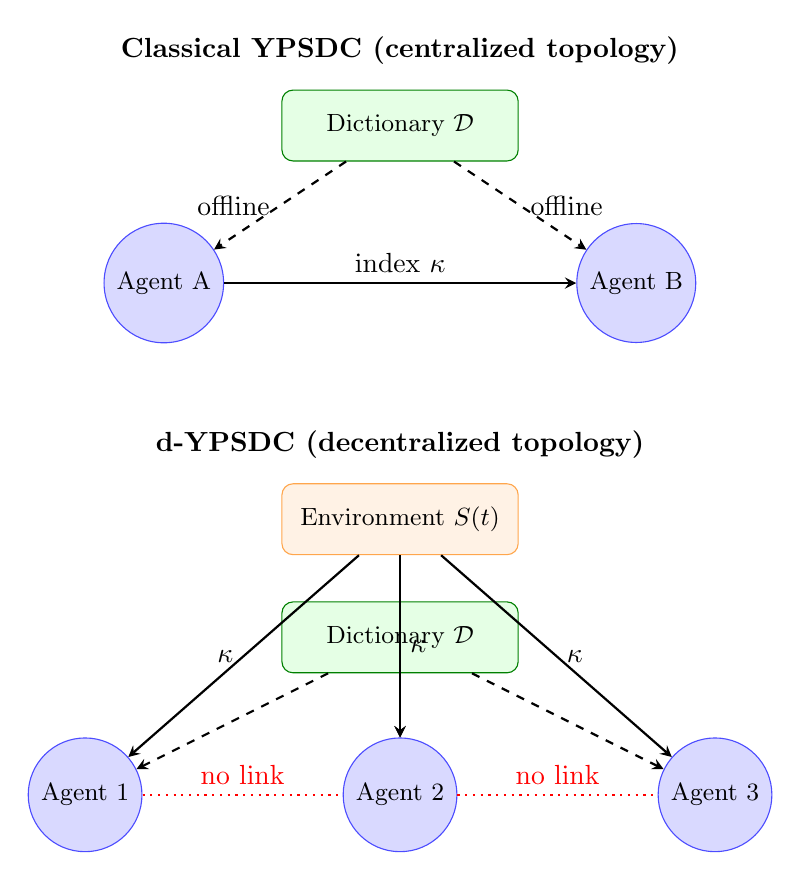
\begin{tikzpicture}[
			agent/.style={circle, draw=blue!70, fill=blue!15, minimum size=1.2cm, font=\small},
			dict/.style={rectangle, draw=green!50!black, fill=green!10, rounded corners, minimum width=3cm, minimum height=0.9cm, font=\small},
			env/.style={rectangle, draw=orange!70, fill=orange!10, rounded corners, minimum width=3cm, minimum height=0.9cm, font=\small},
			arrow/.style={->, >=stealth, thick},
			dashedarrow/.style={->, >=stealth, thick, dashed},
			]
			
			% ---- Classical YPSDC (top) ----
			\begin{scope}[local bounding box=classic]
				\node[dict] (dict1) at (0,0) {Dictionary \(\mathcal{D}\)};
				\node[agent] (A1) at (-3, -2) {Agent A};
				\node[agent] (A2) at (3, -2) {Agent B};
				\draw[dashedarrow] (dict1) -- (A1) node[midway, left] {offline};
				\draw[dashedarrow] (dict1) -- (A2) node[midway, right] {offline};
				\draw[arrow] (A1) -- (A2) node[midway, above] {index \(\kappa\)};
			\end{scope}
			\node[above=0.2cm of classic.north, font=\bfseries] {Classical YPSDC (centralized topology)};
			
			% ---- d‑YPSDC (bottom) ----
			\begin{scope}[local bounding box=decentr, yshift=-6cm]
				\node[env] (env) at (0,1) {Environment \(S(t)\)};
				\node[dict] (dict2) at (0,-0.5) {Dictionary \(\mathcal{D}\)};
				\node[agent] (B1) at (-4, -2.5) {Agent 1};
				\node[agent] (B2) at (0, -2.5) {Agent 2};
				\node[agent] (B3) at (4, -2.5) {Agent 3};
				\draw[arrow] (env) -- (B1) node[midway, left] {\(\kappa\)};
				\draw[arrow] (env) -- (B2) node[midway, right] {\(\kappa\)};
				\draw[arrow] (env) -- (B3) node[midway, right] {\(\kappa\)};
				\draw[dashedarrow] (dict2) -- (B1);
				\draw[dashedarrow] (dict2) -- (B2);
				\draw[dashedarrow] (dict2) -- (B3);
				% Explicitly indicate the absence of links between agents
				\draw[red, thick, dotted] (B1) -- (B2) node[midway, above, red] {no link};
				\draw[red, thick, dotted] (B2) -- (B3) node[midway, above, red] {no link};
			\end{scope}
			\node[above=0.2cm of decentr.north, font=\bfseries] {d‑YPSDC (decentralized topology)};
			
		\end{tikzpicture}
		\caption{Comparison of topologies. In the classical YPSDC, agent A actively sends an index to agent B. In the decentralized d‑YPSDC, all agents simultaneously read the same index from the environment and exchange no messages.}
		\label{fig:topology}
	\end{figure}
	
	\section{Examples of d‑YPSDC in Various Systems}
	
	\subsection{Biology: flocking behavior and “tacit consent”}
	
	Synchronous collective actions (sudden turns of a fish school, simultaneous take‑off of a bird flock, freezing of ground squirrels) are observed in many animal species without acoustic or visual signals specific to each group member. Instead, all individuals \textbf{simultaneously perceive} a change in some environmental parameter — a gust of wind, the shadow of a predator, a change in illumination — and react in accordance with an innate (genetic) dictionary.
	
	The example of human hair, discussed earlier, also fits into this scheme: long scalp hair can serve as a highly sensitive detector of air flows and temperature, enabling a group of people to synchronously register a change in the weather without exchanging words.
	
	\subsection{Economics and finance}
	
	The release of a key macroeconomic indicator (for instance, the US unemployment rate) triggers an instant and coherent reaction from millions of market participants. Traders do not communicate with one another; they use a shared “dictionary” — trading algorithms, economic models, or simply expectations formed by previous experience. The index (the numerical value of the indicator) is delivered by the environment (information terminals) to all of them simultaneously, and the market moves as a single entity.
	
	\subsection{Blockchain and smart contracts}
	
	Decentralized applications (dApps) often rely on \textbf{oracles} — external data sources that supply information about the real world to the blockchain. The smart contract plays the role of a dictionary distributed among all network nodes. When the oracle publishes an index (for example, the ETH/USD exchange rate at time \(t\)), all nodes simultaneously activate the corresponding branch of the contract without additional consensus. This is a pure implementation of d‑YPSDC in a digital environment.
	
	\subsection{Quantum entanglement}
	
	Perhaps the most profound physical realization of d‑YPSDC occurs in quantum mechanics. Consider a pair of entangled particles. Their shared wave function is a dictionary that prescribes the correlations between possible measurement outcomes. When a measurement is performed on one particle, its result can be regarded as an \textbf{environmental index} that is simultaneously accessible to the second particle thanks to the non‑local properties of the quantum field. The second particle “activates” the correlated state without receiving any classical signal. Within d‑YPSDC this is interpreted as a synchronous reading of the same index from a common physical medium (the quantum field), requiring no transmission of information between the particles.
	
	\section{Ontological Foundation: Matter as Coordination, Geometry as a Consequence}
	
	The principal difference between YUCT and standard field theories is that \textbf{the coordination field does not exist in an empty space‑time}. On the contrary, space‑time itself is a secondary, emergent manifestation of a more fundamental reality — a network of coordinating elements. This postulate has two key consequences that directly apply to the decentralized YPSDC.
	
	\textbf{1. Matter = coordination.} The notion of an “elementary particle” or “agent” is not independent of the coordination process. An element exists only insofar as it participates in coordination acts and can be identified through its dictionary. Outside the coordination network there is no matter; only formal mathematical points devoid of physical content remain. In the context of d‑YPSDC this means that the agents reading the environmental index are not passive observers — their very existence as coherently acting units \emph{creates} the coordination field \(\Psi_{MN}\) that subsequently delivers indices to them.
	
	\textbf{2. Geometry does not exist without matter.} The rotating‑disk paradox (known in the literature as the Ehrenfest paradox) demonstrates that spatial geometry cannot be given \emph{a priori} but is determined by the state of motion and the internal cohesive forces of the material body. In YUCT this is generalized to the statement that the space‑time metric \(g_{\mu\nu}(x)\) is an \emph{effective} quantity that emerges from averaging over coordination interactions. Where coordination is absent (\(K_{\mathrm{eff}} \to 1\)), geometry degenerates and loses its operational meaning. In d‑YPSDC this manifests itself in the fact that the effective “conductivity” of the environment for the index depends on the density and connectivity of the coordinating agents, not on the properties of some absolute space.
	
	Thus, \textbf{the environment that delivers the index is not a passive container but the coordination field itself, generated by material agents}. It is the presence of agents with a shared dictionary that “switches on” the field \(\Psi_{MN}\) and endows it with the structure that enables synchronous delivery of indices. In the absence of agents (or when the dictionary is destroyed) the field returns to a symmetric, uncoordinated state, equivalent to the absence of classical space‑time. This fully corresponds to the picture in which space, time, and matter are three inseparable aspects of a single coordination process.
	
	\section{Mathematical Model of d‑YPSDC in the 19‑dimensional Space of YUCT}
	\label{sec:math-model}
	
	\subsection{The 19‑dimensional coordination field and its action}
	
	The fundamental arena of YUCT is a 19‑dimensional pseudo‑Riemannian manifold \(\mathcal{M}_{19}\) with metric \(G_{MN}\) of signature \((+,-,\dots,-)\). It is foliated over the four‑dimensional space‑time \(M_4\):
	\begin{equation}
		\mathcal{M}_{19} = M_4 \times F_{15},
	\end{equation}
	where \(F_{15}\) is a compact internal space of coordination degrees of freedom. The key field is the \textbf{coordination field} \(\Psi_{MN}(X)\), which encodes the distributed dictionary and the index‑carrying medium. The simplest action has the form
	\begin{equation}
		S_{19} = \frac{1}{2\kappa_{19}} \int d^{19}X \sqrt{-G}\, R(G) + \int d^{19}X \sqrt{-G}\, \mathcal{L}_{\mathrm{coord}},
		\label{eq:S19}
	\end{equation}
	where the curvature \(R(G)\) provides the background geometry, and the coordination Lagrangian is
	\begin{equation}
		\mathcal{L}_{\mathrm{coord}} = -\frac{1}{4} \Tr(\Psi_{MN}\Psi^{MN}) + \frac{1}{2} G^{MN}\,\partial_M \phi\,\partial_N \phi - V(\phi)
		\label{eq:Lcoord}
	\end{equation}
	containing the gauge field \(\Psi_{MN}\) (an analogue of the coordination‑interaction strength) and the scalar \(\phi = \ln(K_{\mathrm{eff}}/K_0)\), which parametrizes the local coordination efficiency.
	
	\subsection{Introducing agents and the dictionary}
	
	Agents \(A_i\), \(i=1,\dots,N\), are represented as point‑like sources localized in \(M_4\) and “smeared” over \(F_{15}\) according to their dictionary profile. Each agent possesses a \textbf{dictionary function} \(f_{\mathcal{D}}^{(i)}(\kappa)\) that maps the index \(\kappa \in \mathcal{E}\) to the desired action. The interaction of the agents with the field \(\Psi_{MN}\) is given by the term
	\begin{equation}
		S_{\mathrm{int}} = \sum_{i=1}^{N} \int d\tau_i \left[ \frac{1}{2} m_i \dot a_i^2 - \lambda_i \bigl( a_i - f_{\mathcal{D}}^{(i)}(\kappa) \bigr)^2 \right],
		\label{eq:Sint}
	\end{equation}
	where \(a_i\) is the action actually performed, and \(\tau_i\) is the proper time of the agent. The index \(\kappa\) here is not an external parameter but the value of the field \(\Psi_{MN}\) (or its projection onto \(M_4\)) at the agent’s location:
	\begin{equation}
		\kappa(x_i) = \int_{F_{15}} d^{15}Y \sqrt{-G^{(15)}}\, \mathcal{O}[\Psi_{MN}](x_i, Y),
		\label{eq:kappa}
	\end{equation}
	where \(\mathcal{O}\) is some operator that projects the coordination field onto the index space. In the simplest case \(\mathcal{O}[\Psi] = \Tr(\Psi)\) or simply \(\phi\).
	
	\subsection{Equations of motion and index delivery}
	
	Varying the total action \(S_{19} + S_{\mathrm{int}}\) with respect to \(\Psi_{MN}\) yields the equation
	\begin{equation}
		D_M \Psi^{MN} = J^{N}_{\mathrm{coord}},
		\label{eq:Psi-eq}
	\end{equation}
	where \(J^{N}_{\mathrm{coord}}\) is the total coordination current of the agents:
	\begin{equation}
		J^{N}_{\mathrm{coord}}(X) = \sum_{i=1}^{N} \int d\tau_i\, \frac{\delta^{(19)}(X - X_i(\tau_i))}{\sqrt{-G}}\, \frac{\partial \mathcal{L}_{\mathrm{int}}}{\partial (\partial_N \Psi)}.
	\end{equation}
	For slowly varying fields and a static dictionary the effective equation reduces to a wave equation on \(M_4\) with sources:
	\begin{equation}
		\Box \phi - m_{\mathrm{eff}}^2 \phi = \sum_{i} g_i \delta^{(4)}(x - x_i),
		\label{eq:phi-eq}
	\end{equation}
	where \(m_{\mathrm{eff}}^2 = V''(0)\), and the coupling constants \(g_i\) are proportional to the “loudness” of the index.
	
	The solution of Eq.~(\ref{eq:phi-eq}) in the quasi‑static approximation is
	\begin{equation}
		\phi(x) = \sum_i g_i \, G_{\mathrm{ret}}(x, x_i),
	\end{equation}
	with \(G_{\mathrm{ret}}\) the retarded Green’s function for a massive scalar field. If all agents are situated in a region whose size is much smaller than the Compton wavelength \(\lambda_c = 1/m_{\mathrm{eff}}\), then \(\phi(x)\) is practically identical at all points \(x_i\). This explains the \textbf{simultaneous reading of the same index} by all agents: the index, produced by the environment (i.e.\ by boundary conditions or a cosmological background), propagates through \(M_4\) and, being long‑wavelength, appears identical to all local observers.
	
	Thus, the synchronicity of activation does not require superluminal signals: it is a natural consequence of the fact that the coordination field \(\phi\) behaves as a homogeneous background on the scale of the group. At the same time, each agent interacts exclusively with the field, not with other agents; no direct exchange of information takes place, which is the essence of the decentralized YPSDC.
	
	\subsection{Connection with the efficiency \(K_{\mathrm{eff}}\)}
	
	Local coordination efficiency is defined as the ratio of the information capacity of the dictionary to the index length. In terms of the field \(\phi\):
	\begin{equation}
		K_{\mathrm{eff}}(x) = K_0 e^{\phi(x)},
		\label{eq:Keff-field}
	\end{equation}
	where \(K_0 \approx 1\) is the background value in the vacuum (absence of coordinated agents). The environmental delivery of an index creates a perturbation \(\delta\phi\), so that in the region occupied by the agents
	\begin{equation}
		K_{\mathrm{eff}}^{\mathrm{(d)}} = K_0 \exp\!\left( \sum_i g_i G_{\mathrm{ret}}(x, x_i) \right).
	\end{equation}
	For a group of \(N\) identical agents located within a volume \(V \ll \lambda_c^3\),
	\begin{equation}
		K_{\mathrm{eff}}^{\mathrm{(d)}} \approx K_0 \exp\!\left( \frac{N g}{4\pi} \frac{e^{-m_{\mathrm{eff}} r_0}}{r_0} \right),
	\end{equation}
	where \(r_0\) is the characteristic distance between agents. Because \(N g > 0\) (the index enhances coordination), the value of \(K_{\mathrm{eff}}^{\mathrm{(d)}}\) can significantly exceed unity for large \(N\) or strong coupling \(g\).
	
	This demonstrates directly that \textbf{the decentralized YPSDC provides \(K_{\mathrm{eff}} \gg 1\) without any exchange of indices within the group}. The growth of efficiency is exclusively due to the geometry of the field \(\phi\): all agents are immersed in a common coordination field that, being excited by an external index, simultaneously activates their dictionaries.
	
	\section{Two Regimes of the Same Protocol: Centralized vs.\ Decentralized YPSDC}
	\label{sec:two-regimes}
	
	The examples and the mathematical model presented above might create the impression that
	d‑YPSDC is a fundamentally new coordination protocol. It is not. Ontologically, there is
	only \textbf{one YPSDC mechanism}: the coordination field $\Psi_{MN}$ carries indices, and
	all agents interact exclusively with this field, activating entries of a shared
	\emph{a‑priori} dictionary. The distinction between ``centralized'' YPSDC and
	``decentralized'' d‑YPSDC is purely phenomenological and reflects the dominant source
	of the coordination current $J^{N}_{\mathrm{coord}}$ that appears in the field equations
	(see Appendix~A of \cite{YUCT}).
	
	\subsection{Two Regimes}
	\begin{enumerate}[leftmargin=*, label=\textbf{(\arabic*)}]
		\item \textbf{Centralized regime (classical YPSDC).} The current $J^{N}_{\mathrm{coord}}$
		is dominated by a localized agent (the sender). That agent actively excites the field,
		creating a propagating perturbation that reaches one or more designated receivers.
		This regime describes point‑to‑point or star‑topology communication (e.g.\ a GSM
		tower broadcasting to mobile phones, or the GMT time signal).
		
		\item \textbf{Decentralized regime (d‑YPSDC).} The localized currents of individual
		agents are negligible compared to a global, slowly varying background --- an
		environmental mode of $\Psi_{MN}$. The background provides an index that is
		simultaneously accessible to all agents. This regime describes quantum entanglement,
		flocking behaviour, quorum sensing, the reaction of financial markets to macroeconomic
		indicators, and the activation of smart contracts by blockchain oracles.
	\end{enumerate}
	
	\subsection{Transition between the Regimes}
	The dimensionless parameter
	\[
	\Theta = \frac{|J_{\mathrm{agent}}|}{|J_{\mathrm{env}}|},
	\]
	where $J_{\mathrm{agent}}$ is the current produced by the strongest individual sender and
	$J_{\mathrm{env}}$ is the effective current of the environmental background, controls the
	crossover between the two regimes:
	\[
	\begin{cases}
		\Theta \gg 1 & \text{centralized regime (classical YPSDC)}, \\
		\Theta \ll 1 & \text{decentralized regime (d‑YPSDC)}, \\
		\Theta \sim 1 & \text{mixed behaviour}.
	\end{cases}
	\]
	
	\subsection{Ontological Status}
	d‑YPSDC requires \textbf{no extra fields, no modification of the Lagrangian, and no
		revision of the ontological primitives} of YUCT. The 19‑dimensional action
	$S_{19}$ and the observer fields $\phi_1,\phi_2$ (Appendix~A) already contain
	everything necessary for both regimes. The term ``d‑YPSDC'' is retained only
	as a convenient phenomenological label for the ubiquitous class of phenomena in
	which coordination is achieved without an identifiable active sender.
	
	This clarification is essential for the logical completeness of the YUCT framework:
	the theory describes all forms of coordination --- from explicit human communication to
	the non‑local correlations of quantum mechanics --- through a \emph{single} protocol
	applied to a \emph{single} coordination field.
	
	\subsection{Example: quantum entanglement as d‑YPSDC}
	
	In the quantum case the dictionary is the shared wave function \(\Psi_{AB}\) of an entangled pair. Choose the operator \(\mathcal{O}\) in (\ref{eq:kappa}) so that the index \(\kappa\) coincides with the outcome of a measurement on the first particle. Then Eq.~(\ref{eq:phi-eq}) describes the propagation of this outcome (via the coordination field \(\phi\)) to the second particle. Because the field is massive and static, the correlation is established instantaneously in the sense of synchronous activation, but without energy transfer. This is the geometric interpretation of Bell‑inequality violation in YUCT.
	
	Mathematically, the degree of violation \(S\) is expressed through the efficiency:
	\begin{equation}
		S = 2\sqrt{2} \frac{K_{\mathrm{eff}}^{\mathrm{(d)}}}{K_{\mathrm{eff}}^{\mathrm{(d)}} + 1},
	\end{equation}
	so that the maximal quantum value \(2\sqrt{2}\) is reached when \(K_{\mathrm{eff}}^{\mathrm{(d)}} \to \infty\) (ideal dictionary), while the correlations disappear when \(K_{\mathrm{eff}}^{\mathrm{(d)}} \to 1\) (destruction of the dictionary).
	
	This model unifies biology, economics, and quantum physics within the common equations (\ref{eq:Psi-eq})--(\ref{eq:Keff-field}), demonstrating the universality of the coordination field \(\Psi_{MN}\) and of the d‑YPSDC protocol.
	
	\section{The Coordination Field as a Universal Carrier of Indices}
	
	If d‑YPSDC is valid for quantum systems, biological populations, and social networks, it is natural to assume the existence of a unified \textbf{coordination field} — a universal medium that:
	
	\begin{itemize}
		\item stores the “universal dictionary” of the laws of nature (symmetries, constants, equations of motion);
		\item delivers indices (measurement outcomes, fluctuations, external influences) simultaneously to all elements of the system;
		\item ensures the synchronicity of activation observed as quantum non‑locality, collective behavior, or rapid market response.
	\end{itemize}
	
	In this context, classical communication (the transmission of a signal from one agent to another) turns out to be a \textbf{special case} that arises when the environment is incapable of delivering the index to all agents simultaneously (e.g., because of a high noise level), forcing the agents to duplicate the index by means of direct communication.
	
	This hypothesis does not contradict relativity, because no energy or information is transmitted faster than light: the index propagates through the environment at a speed not exceeding \(c\) and becomes accessible to all agents only after reaching their local vicinity. The synchronicity of activation is exclusively due to the common dictionary and the identity of the index, not to superluminal signaling.
	
	\section{Conclusion}
	
	We have introduced the concept of the decentralized YPSDC (d‑YPSDC) — a protocol in which coordination is achieved through the simultaneous reading of a common environmental index by all agents, using a pre‑distributed a‑priori dictionary. This scheme explains a broad range of phenomena — from biological synchronization to quantum non‑locality — without invoking any hidden communication.
	
	The d‑YPSDC naturally leads to the notion of a \textbf{coordination field} as the fundamental entity responsible for the universal consistency of natural processes. The mathematical model based on the 19‑dimensional action of YUCT demonstrates that decentralized coordination arises from the unified equations of the field \(\Psi_{MN}\), and that the efficiency \(K_{\mathrm{eff}}\) grows exponentially with the number of agents and the coupling strength. The further formalization of this field and its connection to quantum theory and general relativity constitutes a program for future research.
	
	\begin{thebibliography}{9}
		\bibitem{YUCT} A.~V.~Yakushev, \emph{Yakushev Unified Coordination Theory (YUCT)}, Zenodo, DOI:10.5281/zenodo.18444599 (2026).
		\bibitem{AppendixB} A.~V.~Yakushev, Appendix B: Temporal Coordination Paradox, in \emph{YUCT} (2026).
		\bibitem{Blockchain} S.~Nakamoto, ``Bitcoin: A Peer-to-Peer Electronic Cash System'' (2008).
		\bibitem{Ben-Jacob} E.~Ben-Jacob, ``Bacterial self-organization: co-enhancement of complexification and adaptability'', \emph{Physica A} (2003).
		\bibitem{EPR} A.~Einstein, B.~Podolsky, N.~Rosen, ``Can Quantum-Mechanical Description of Physical Reality Be Considered Complete?'', \emph{Phys. Rev.} \textbf{47}, 777 (1935).
	\end{thebibliography}
	
\end{document}